\documentclass[border=2mm]{standalone}
\usepackage{tikz}
\begin{document}

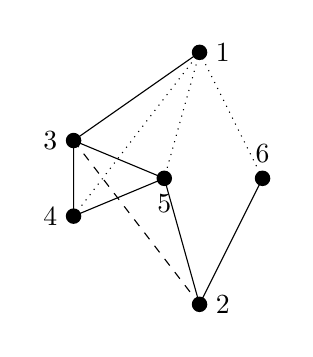
\begin{tikzpicture}[scale=0.8, inner sep=2mm]
  % Define all node coordinates in numerical order for clarity
  \coordinate (1) at (2, 2);   % Top-right node
  \coordinate (2) at (2, -2);  % Bottom-right node
  \coordinate (3) at (0, 0.6); % Upper-left node
  \coordinate (4) at (0, -0.6);% Lower-left node
  \coordinate (5) at (1.44, 0);% Mid-left node
  \coordinate (6) at (3, 0);   % Rightmost node

  % Draw solid edges (avoiding duplicates)
  \draw (5) -- (3) node[left] {3}
        -- (4) node[left] {4}
        -- (5) node[below] {5}
        -- (2) node[right] {2}
        -- (6) node[above] {6}; % label 6 placed above for clarity

  % Complete the main polygonal connections
  \draw (3) -- (1) node[right] {1};

  % Draw dashed and dotted auxiliary edges
  \draw[dashed] (3) -- (2);                % Diagonal dashed edge
  \draw[dotted] (4) -- (1) -- (5);         % Dotted path from 4 to 5 via 1
  \draw[dotted] (1) -- (6);                % Dotted edge from 1 to 6

  % Draw all node points
  \foreach \i in {1,...,6} {
    \fill (\i) circle (3.5pt);
  }
\end{tikzpicture}

\end{document}
